\title{Midterm 3 for Calculus-Based Physics-1: Mechanics (PHYS150-01)}
\author{Dr. Jordan Hanson - Whittier College Dept. of Physics and Astronomy}
\date{November 6th, 2017}
\documentclass[10pt]{article}
\usepackage[a4paper, total={18cm, 27cm}]{geometry}
\usepackage{outlines}
\usepackage[sfdefault]{FiraSans}
\usepackage{graphicx}

\begin{document}
\maketitle

\section{Definition of Work}
\begin{enumerate}
\item \textit{In each of the following three questions, determine whether work is being performed \textbf{on the briefcase} by the man}.
\begin{itemize}
\item A man is walking horizontally, carrying a briefcase at a constant height. \textbf{(a)} No work is done on briefcase \textbf{(Displacement is not in the direction of the force).} (b) Positive work is done on briefcase (c) Negative work is done on briefcase
\item A man stands still, and holding a briefcase in a fixed position.  \textbf{(a)} No work is done on briefcase \textbf{(The displacement is zero, even though the force is not).} (b) Positive work is done on briefcase (c) Negative work is done on briefcase
\item A man stands still, and lowers the briefcase to a height less than the original height.  (a) No work is done on briefcase (b) Positive work is done on briefcase \textbf{(c)} Negative work is done on briefcase \textbf{(The displacement is in the same direction of the force of gravity, but we want the work done by the man, not gravity).}
\item A man raises the briefcase to a height greater than the original height.  (a) No work is done on briefcase \textbf{(b)} Positive work is done on briefcase \textbf{(The force by the man is against gravity and in the same direction as the displacement).} (c) Negative work is done on briefcase
\end{itemize}
\item For this problem, use the work formula $W = \vec{F}_{\rm Net} \cdot \vec{x}$.  (a) Draw the correct free-body diagram for a crate being pushed horizontally against friction by some applied force $\vec{f}$.  (b) Calculate the work done by $\vec{F}_{\rm Net}$ on a 200 kg palette crate through a distance $\vec{x} = 10$ m on a surface with coefficient of kinetic friction of 0.05, if $\vec{f} = 150\hat{i}$ N (in the horizontal direction).  \\
\begin{figure}[ht]
\centering
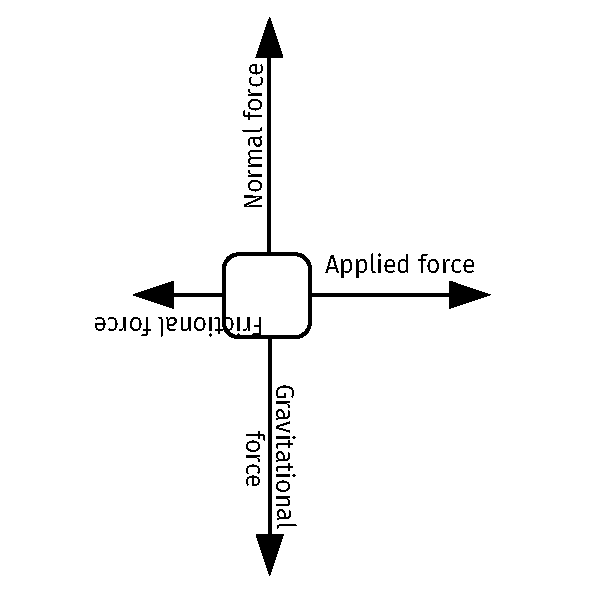
\includegraphics[width=0.2\textwidth]{figures/Friction1.pdf}
\end{figure} \\
$\vec{F}_{\rm net} = 150\hat{i} - 0.05(200)10\hat{i} = 50\hat{i}$ N, so $W = 50(10)$ N m = 500 J.
\item A crane lifts a shipping container from a ship to the dock.  The shipping container is at a height of 30 meters above the water initially, and ends 4 meters above the water after the move is complete.  The shipping container has a mass of 4500 kg.  (a) Draw the correct free-body diagram.  (b) What is the work done on the shipping container, in kJ?  Should it be positive or negative? (\textit{Recall that the work done lifting an object a height $h$ against gravity is $W = mgh$}).\\
\begin{figure}[hb]
\centering
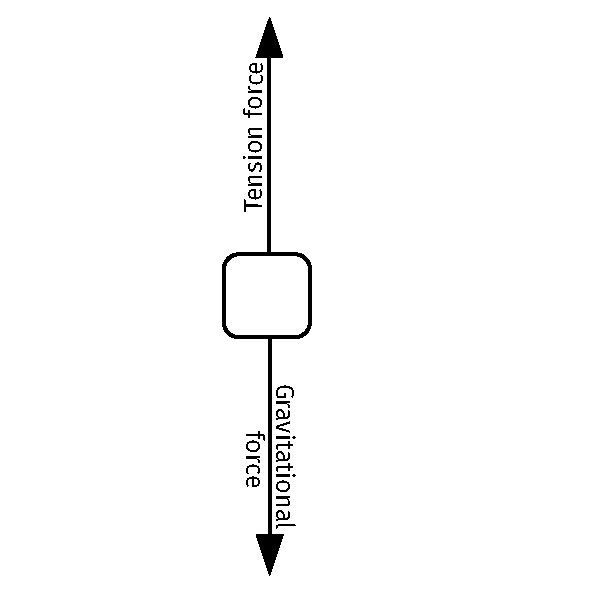
\includegraphics[width=0.2\textwidth]{figures/Crane1.pdf}
\end{figure} \\
$W = \vec{F} \cdot \vec{x} = -mg\hat{j} \cdot (-26) \hat{j}$ N m = 1200 kJ.  However, the work done by the crane is -1200 kJ.
\end{enumerate}
\section{Kinetic Energy}
\begin{enumerate}
\item In a particular radioactive isotope, \textit{thermal neutrons} are emitted with kinetic energy $KE = \frac{1}{2}mv^2$.  If the mass of a neutron is $1.7\times 10^{-27}$ kg, and the velocity is $v = 3\times 10^6$ m/s, (a) what is the kinetic energy? (b) If 1 electron-Volt equals $1.6 \times 10^{-19}$ Joules, how many electron-Volts of energy do these neutrons have? \\ $KE \approx \frac{1}{2}(2 \times 10^{-27}) (3 \times 10^8)^2 \approx 10^{-14}$ J.  In eV, this is $10^{-14}/(2 \times 10^{-19}) \approx 0.05 \times 10^6 = 0.05$ MeV.
\item Not every particle in the radiation is a neutron.  Suppose one is an \textit{alpha-particle}, which has four times the mass of a neutron.  If we detect an alpha particle that has the same speed as a neutron, and the neutron has kinetic energy of 5 MeV ($5 \times 10^{6}$ electron-Volts), what is the kinetic energy of the alpha particle? \\
\textbf{This problem was meant to be a scaling problem, but some of you assumed the energy from the previous part and did it that way.  I gave full points either way if you made no mistake.} If the energy is 5 MeV, but then we quadruple the mass, then the energy must quadruple, so 20 MeV.  (Kinetic energy is directly proportional to the mass).
\end{enumerate}
\section{Work-Energy Theorem}
\begin{enumerate}
\item An archer's bow acts like a spring with a spring constant of $k=350$ N/m.  If an arrow is loaded into this bow, how much energy is required to draw it back 0.5 m?
\begin{itemize}
\item 4 J
\item \textbf{40 J.}  $W = \frac{1}{2}kx^2 = \frac{1}{2}(350)\left(\frac{1}{2}\right)^2 \approx 350/8$ J.
\item 400 J
\item 4000 J
\end{itemize}
\item Assume all of the energy in the drawn bow in the previous question is released into the kinetic energy of the arrow (mass = 0.02 kg).  If the arrow is fired from a height of 1.5 m, how far does it travel before it lands?
\begin{itemize}
\item 3 m
\item \textbf{30 m.}  This is a kinematics problem.  The time an object takes to fall 1.5 meters may be derived from $\Delta y = -\frac{1}{2}gt^2$, with $\Delta y = -1.5 m$, and $g = 10$ m/s$^2$.  The time is $t = \sqrt{\frac{3}{10}}$.  If all of the work done to draw the bow is dumped into the arrow, we have $KE = \frac{1}{2}mv^2$, or $v = \sqrt{\frac{2KE}{m}} = 20\sqrt{10}$ m/s.  If the arrow takes time $t$ to fall, and is travelling horizontally at $v$, then the range is $R = vt$, or $20\sqrt{10}\sqrt{\frac{3}{10}} = 20\sqrt{3} \approx 30$ m.
\item 300 m
\item 3000 m
\end{itemize}
\end{enumerate}
\section{Gravitational Potential Energy}
\begin{enumerate}
\item The height of Freedom Tower in New York City is 1776 feet, or or 541 meters.  Suppose we drop a penny off of the top!  (a) What is the \textit{potential energy} in J before we drop it, if it has a mass of 2.5 grams?
\begin{itemize}
\item 1.35 J
\item \textbf{13.5 J.}  Recall that the gravitational potential energy is $U = mgh$, for an object displaced a height $h$ above the ground.  We have $U = 2.5 \times 10^{-3} (10) 5.4 \times 10^{2} = 2.5(5.4) = 13.5$ J
\item 27 J
\item 54 J
\end{itemize}
(b) What velocity does the penny have when it hits the street, assuming no drag force?
\begin{itemize}
\item 1 m/s
\item 10 m/s
\item \textbf{100 m/s.}  The easiest way to get this is to say that all of the potential energy becomes kinetic energy: $mgh = \frac{1}{2}mv^2$, leading to $v = \sqrt{2gh} = \sqrt{2(10)(540)} \approx \sqrt{10^4} = 100$ m/s.  We can also find $v = \sqrt{2gh}$ from the kinematic equation $v^2 = v_{\rm i}^2 - 2g\Delta y$, by noticing that $v_{\rm i} = 0$.
\item 300 m/s
\end{itemize}
\end{enumerate}
\section{Conservative Forces}
\begin{enumerate}
\item (a) Which of these forces is \textit{conservative}?
\begin{itemize}
\item \textbf{The spring force (Hooke's Law)} The work done in displacing an oscillator like a spring with constant $k$ by a displacement $x$ is $W = \frac{1}{2}kx^2$.  If we return to the same $x$, the displacement is zero and therefore $W$ is zero.
\item Kinetic friction.  This is not conservative.  If an object is returned to the same position, work will have been done on it regardless, because the force of friction changes direction to always be in opposition to the direction of motion (the force of an oscillator does not do this).
\item Drag due to air.  This is not conservative, for the same reasons as kinetic friction.
\item Stoke's Law (drag in viscous substances) This is not conservative, for the same reasons as kinetic friction.
\end{itemize}
(b) In your own words, define a \textit{conservative} force. \\
Any of these ideas is right:
\begin{itemize}
\item Work is path independent.
\item Returning to the same position means no net work.
\item The y-derivative of the x-component is the x-derivative of the y-component.
\item $\oint \vec{F} \cdot d\vec{r} = 0$.
\end{itemize}
\end{enumerate}
\end{document}